\section{Protocol}
This protocol will describe the present study, which consist of two experiments testing pain tolerance and pain threshold after practicing mindfulness meditation or after not practicing mindfulness meditation. 

\subsection{Purpose}
The treatment of chronic pain has constraints, as the treatments are only relieving the pain instead of curing the pain. Another issue is that some of these treatments, example medication, have side effect, as described in \ref{sec:xxx}. 

There is alternative to medication such as yoga, hypnosis and mindfulness, which have shown to have an influence on relieving pain.

An alternative to the present treatment is mindfulness meditation, as described in \ref{sec:xxx}. 

In order to investigated the influence of mindfulness meditation on pain threshold and pain tolerance following hypothesis is proposed:
\vspace{-.5cm}
\begin{itemize}
\item Short-term mindfulness meditation increases the pressure pain threshold and the pressure pain tolerance.
\end{itemize}

\subsection{Subjects}
Forty healthy subjects were recruited for the experiment, 20 males (M) and 20 females (F) with a mean age $\pm$XX. A homogeneous group of participants were enrolled in order to limit the amount of variables in the study. For insuring this, specific inclusion and exclusion criteria have been formed for this experiment. 

\textbf{Inclusion criteria:}
\vspace{-.5cm}
\begin{itemize}
	\item Healthy subjects age between 20-30 years
	\vspace{-.3cm}
	\item Must have time to meditate for 4-5 days, 30 minutes per day.
	\vspace{-.3cm}
	\item Normal BMI (F: 19-24 M: 20-25)
\end{itemize}

\textbf{Exclusion criteria:}
\vspace{-.5cm}
\begin{itemize}
	\item Ongoing meditation practice 
	\vspace{-.3cm}
	\item Acute or chronic pain
	\vspace{-.3cm}
	\item Pregnancy 
	\vspace{-.3cm}
	\item Neurological, musculoskeletal or mental illness
	\vspace{-.3cm}
	\item Signs or symptoms of any serious systemic diseases 
	\vspace{-.3cm}
	\item Psychiatric, analgesic or other medications that might influence their response to pain 
		\vspace{-.3cm}
	\item Abusive drug or alcohol use
		\vspace{-.3cm}
	\item Lack of ability to cooperate
\end{itemize}

\vspace{-.5cm}
Furthermore, is it not necessary that subjects believe in the effect of mindfulness meditation.\fxnote{I don't know about this sentence, i think it does not fit in here. Maybe it is more something we should write for the participants or could we put it in as one of our criteria?.}

\subsection{Setup}
The Pressure Pain Threshold (PPT), defined as the pressure at which the sensation changed from pressure to pain, has been recognized as an effective and reliable way to quantify pain measures. In this study PPT was measured using (our ALGOMETER). PPT were measured in the upper trapezius. Testing points were marked to ensure reliable and rapid location during the experimental procedure. 
The algometer was applied four times, two on the left side and two on the right side of the upper trapezius, and the average of the registrations was filed. The subjects had a 5 minutes resting time between measurements. PPT values were measured two times, the first day of the study and after 4-5 days since the first measure.

\subsection{Approach}
For this particular experiment a parallel study was conducted. The subjects recruited for the experiment were randomly assigned in two different groups, the control group or the treatment group, with a equal amount of female and males in the groups. The control group consisted of twenty subjects no meditation. The treatment group consisted of twenty subjects meditation. The structure of the study design is illustrated on \figref{fig:studydesign}.


\begin{figure}[H]
	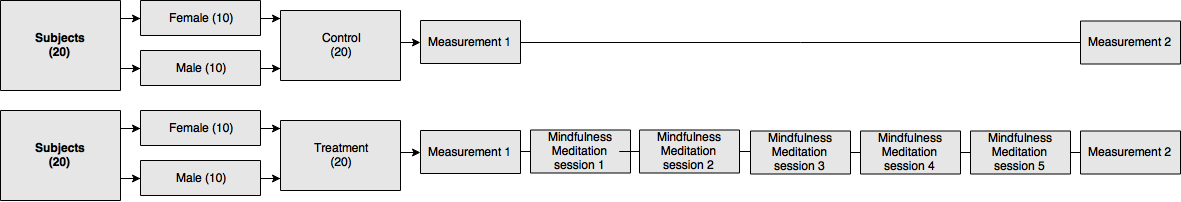
\includegraphics[width=1\textwidth]{figures/studydesign.png} 
	\caption{Parallel study design.}
	\label{fig:studydesign}  
\end{figure}  

\subsection{Procedure}

Control group
Treatment group

\subsubsection{Mindfulness meditation}
Guided meditation for 30 minutes in groups, sitting positions. 